\documentclass[a4paper,12pt]{article}

\usepackage{graphicx}
\usepackage{pdfpages}

\begin{document}

\title{Pengembangan Aplikasi Sampling \\ Penutup Lahan}
\author{Khairil Fahmi Faisal \\ Gemasakti Adzan}
\date{\today}
\maketitle

\section{Ringkasan}
\texttt{Aplikasi Sampling Penutup Lahan} dapat digunakan untuk mendesain dan melabeli sampel untuk proses klasifikasi citra penginderaan jauh dengan teknik \textit{supervised classification machine learning}. Aplikasi ini dibangun pada platform \texttt{Jupyter Notebook} dengan menggunakan beberapa Python package seperti \texttt{ee}, \texttt{geopandas}, \texttt{ipywidgets}, dan \texttt{ipyleaflet}. Secara garis besar aplikasi ini terdiri dari dua tahapan yaitu 1) membangun set data sampel yang distribusinya didasarkan atas hasil K-Means Clustering dengan proporsi jumlah sesuai luas setiap kluster; 2) memberikan label pada setiap titik sampel secara interaktif melalui \textit{map widget} berbasis \texttt{ipyleaflet}. Aplikasi ini dapat digunakan untuk berbagai macam citra multispektral dan hiperspektral. Melalui aplikasi ini pengguna memiliki opsi untuk menampilkan koleksi data dari katalog maupun asset \texttt{Google Earth Engine}. Hal ini akan membuat proses mendesain sampel menjadi efektif dan efisien, karena pengguna tidak perlu mengunduh data terlebih dahulu untuk dibuka pada perangkat lunak RS/GIS. Penulisan dalam platform \texttt{Jupyter Notebook} dapat digunakan sebagai arsip dan pencatatan yang baik dalam sebuah rangkaian penelitian. Selain itu aplikasi ini berkesinambungan dengan proses terkait lainnya dalam skema besar Land Cover Monitoring System yang juga dibangun dalam platform \texttt{Jupyter Notebook}.

\section{Latar belakang}
Pendekatan \textit{machine-learning} dengan teknik \textit{supervised classification} merupakan metode yang banyak dipakai untuk memproduksi peta penutup lahan dari citra multispektral dan hiperspektral. Beberapa metode yang banyak digunakan misalnya metode \textit{spectral distance-based} (Minimum Distance, Maximum Likelihood, Support Vector Machine/SVM); \textit{decision tree-based} (Decision Trees/DT, Classification and Regression Trees/CART, dan Random Forests/RF); dan \textit{neural-based} (Artificial Neural Network, K-Neural Network). Teknik \textit{supervised classification} memerlukan \textit{labelled samples} dalam proses membangun \textit{classifier model}. Setiap sampel akan "dilatih" dengan membangun hubungan antara \textit{labelled samples} dengan statistik dari \textit{predictors} (berupa \textit{image bands}, \textit{transformation index}, maupun hasil \textit{feature engineering} lainnya) dengan metode \textit{supervised classification} di atas. Kualitas \textit{classifier model} dalam memetakan penutup lahan (digambarkan melalui akurasi \textit{training samples} dan \textit{test samples}) sangat bergantung dari kualitas sampel yang digunakan. Oleh karena itu diperlukan dataset sampel yang baik, yang benar-benar merepresentasikan statistik dari suatu tipe penutup lahan.

\textit{Labelled samples} salah satunya dapat diperoleh dari dataset observasi lapangan, misalnya plot sampel dan hasil observasi lapangan. Namun terkadang untuk area pemetaan yang besar, sampel tersebut tidak cukup representatif dari segi kuantitas dan distribusi spasialnya untuk digunakan sebagai sampel dalam model \textit{supervised classification}. Oleh karena itu sampel lebih sering dibangun dengan membuat dataset sampel dengan proses observasi dan digitisasi (berupa titik maupun area) pada citra penginderaan jauh yang relevan digunakan sebagai referensi. Permasalahannya, proses ini seringkali menghasilkan dataset sampel yang tidak cukup ideal untuk model \textit{supervised classification}. Misalnya, banyak sampel yang \textit{redundant} dan secara statistik tidak meliput distribusi nilai piksel keseluruhan secara utuh. Artinya kecenderungan tidak terambilnya "kluster" sampel dengan karakteristik tertentu bisa terjadi.

Solusi yang dapat digunakan untuk mengatasi permasalahan tersebut di atas beberapa di antaranya adalah pendekatan \textit{semisupervised learning} dan \textit{active learning}. Dalam proses \textit{semisupervised learning}, pertama dilakukan proses \textit{unsupervised clustering} untuk mengelompokkan piksel menjadi beberapa kluster. Setiap kluster kemudian diberikan label tipe penutup lahan, beberapa di antaranya mungkin masih berupa percampuran beberapa tipe penutup lahan. Melalui observasi, kluster-kluster yang menggambarkan kelas penutup lahan murni kemudian dijadikan acuan untuk membuat \textit{labelled sampel}. Proses pada \textit{active learning} pada dasarnya juga dilakukan berdasarkan proses \textit{clustering}, namun yang membedakan setiap kluster tersebut kemudian dilatih dengan sejumlah kecil \textit{labelled samples} menggunakan metode \textit{supervised classification} tertentu, misalnya Support Vector Machine (SVM)\cite{patra2012}. \textit{Feature space} kemudian digunakan untuk mengelompokkan objek sampel yang \textit{robust} (hasil \textit{medoid}) dan membuang objek sampel yang ambigu (dalam \textit{feature space} digambarkan sebagai objek yang lokasinya beririsan dengan kluster atau kelas lain).

\section{Tujuan}
Projek ini bertujuan untuk mendesain sebuah aplikasi pembuatan sampel sebagai \textit{input} dalam \textit{supervised classification} dengan mempertimbangkan berbagai permasalahan di atas. Dalam projek ini, pendekatan yang digunakan adalah \textit{semisupervised learning} dengan menggunakan metode K-Means Clustering. Dari setiap kluster yang dihasilkan, sejumlah titik sampel kemudian diambil secara acak dengan jumlah proporsi berdasarkan luas setiap kluster. Proses berikutnya adalah \textit{data labelling}, yaitu memberikan label pada setiap titik sampel tersebut. Aplikasi ini dibuat pada platform \texttt{Jupyter Notebook}, sehingga prosesnya dapat direpetisi dan juga mengakomodasi perubahan yang dapat dilakukan untuk pengembangan atau perbaikan. Aplikasi ini dapat digunakan untuk berbagai citra multispektral maupun hiperspektral, namun dalam projek ini dicontohkan dengan menggunakan liputan citra Landsat 8 OLI.

\section{Aplikasi Sampling Penutup Lahan}
Aplikasi ini terdiri dari dua bagian, yakni \texttt{Sample generator} untuk membuat set data sampel dan \texttt{Sample data labelling} untuk memberikan label pada setiap titik sampel yang telah dibuat secara interaktif. Pengguna dapat memasukkan \textit{input parameter} utamanya berupa \texttt{GEE asset id}, jumlah kluster, dan juga jumlah titik sampel yang ingin dibuat. 

\subsection{\texttt{Sample generator}}
Seperti telah dikemukakan sebelumnya, set data sampel dibangun dengan mempertimbangkan hasil \textit{unsupervised learning} baik untuk distribusi sebaran maupun kuantitasnya. Hal tersebut untuk meminimalisir unsur subjektifitas yang kerap dijumpai ketika sebaran titik sampel dibuat secara manual. Selain itu hal tersebut dilakukan untuk memastikan bahwa sampel mewakili kondisi data secara menyeluruh, yang diwakili oleh representasi kluster hasil \textit{unsupervised learning}.

Metode \textit{unsupervised learning} yang digunakan adalah K-Means Clustering. Pada dasarnya, K-Means Clustering berupaya untuk mengelompokkan set data sampel ke dalam sejumlah kluster/\textit{centroids} (ditentukan sebagai variabel \texttt{k}) berdasarkan kesamaan karakteristik data prediktor (dalam hal ini nilai spektral/piksel citra penginderaan jauh). Setiap data sampel akan dialokasikan pada kluster yang memiliki kemiripan dengannya. Setiap kluster akan memiliki titik pusat kluster yang posisinya akan berubah-ubah hingga menemukan kondisi stabil dan optimal di mana jarak tiap titik dalam sebuah kluster memiliki variasi paling kecil.

Aplikasi ini menggunakan fungsi K-Means Clustering dari package \texttt{ee} (\texttt{ee.Clusterer.WekaKMeans()}) yang diaplikasikan pada set data 10 ribu titik sampel acak. K-Means Clustering dijalankan untuk sejumlah \texttt{k} kluster yang nilainya telah ditentukan pengguna. Dari sejumlah \texttt{k} kluster tersebut kemudian dihitung proporsi luasnya untuk dijadikan dasar dalam membuat \textit{stratified random samples} (\texttt{ee.stratifiedSample()}) yang jumlah total sampelnya ditentukan oleh pengguna. Hasil keluaran berupa set data \textit{unlabelled samples} ini dapat diekspor oleh pengguna ke \texttt{Google Drive} untuk proses berikunya yaitu \textit{data labelling}.

\subsection{\texttt{Sample data labelling}}
Bagian berikutnya dari \texttt{Aplikasi Sampling Penutup Lahan} adalah proses memberikan label pada setiap objek \textit{unlabelled data} hasil \textit{proportionally stratified random sampling} sebelumnya. Pengguna dapat melakukan proses labelisasi secara interaktif dengan mengacu pada visualisasi citra multispektral dan juga \textit{basemaps} citra satelit penginderaan jauh resolusi tinggi. \textit{User interface} yang dibangun pada aplikasi ini terinspirasi dari proses validasi sampel penutup lahan pada LACO-Wiki\footnote{https://www.laco-wiki.net/}. \textit{Widget} peta interaktif akan menampilkan sebuah titik sampel berdasarkan \texttt{unique id} yang bisa diubah oleh pengguna melalui tombol \texttt{Next feature}, \texttt{Prev. feature}, dan juga \texttt{Jump to feature} dengan memasukkan \texttt{unique id} yang diinginkan. 

Pada setiap titik sampel tersebut kemudian pengguna dapat memberikan label penutup lahan melalui \textit{dropdown list} yang pilihannya dapat ditentukan sendiri oleh pengguna (dalam prototipe ini digunakan kelas \texttt{Forest} dan \texttt{No forest}). Pengguna harus meng-klik tombol \textit{trigger} \texttt{Save edit} untuk menyimpan hasil labelisasi. Hasil akhir proses labelisasi ini akan tersimpan dalam format \texttt{geopandas.GeoDataFrame} yang dapat diekspor ke dalam berbagai format (misalnya \texttt{ESRI Shapefiles}) untuk dapat diperbarui lagi. Pengguna dapat mengekspor hasil final ke \texttt{GEE asset} agar dapat diinteraksikan dengan \texttt{ee object} lainnya dalam proses \textit{supervised classification}.

\begin{figure}
\centering
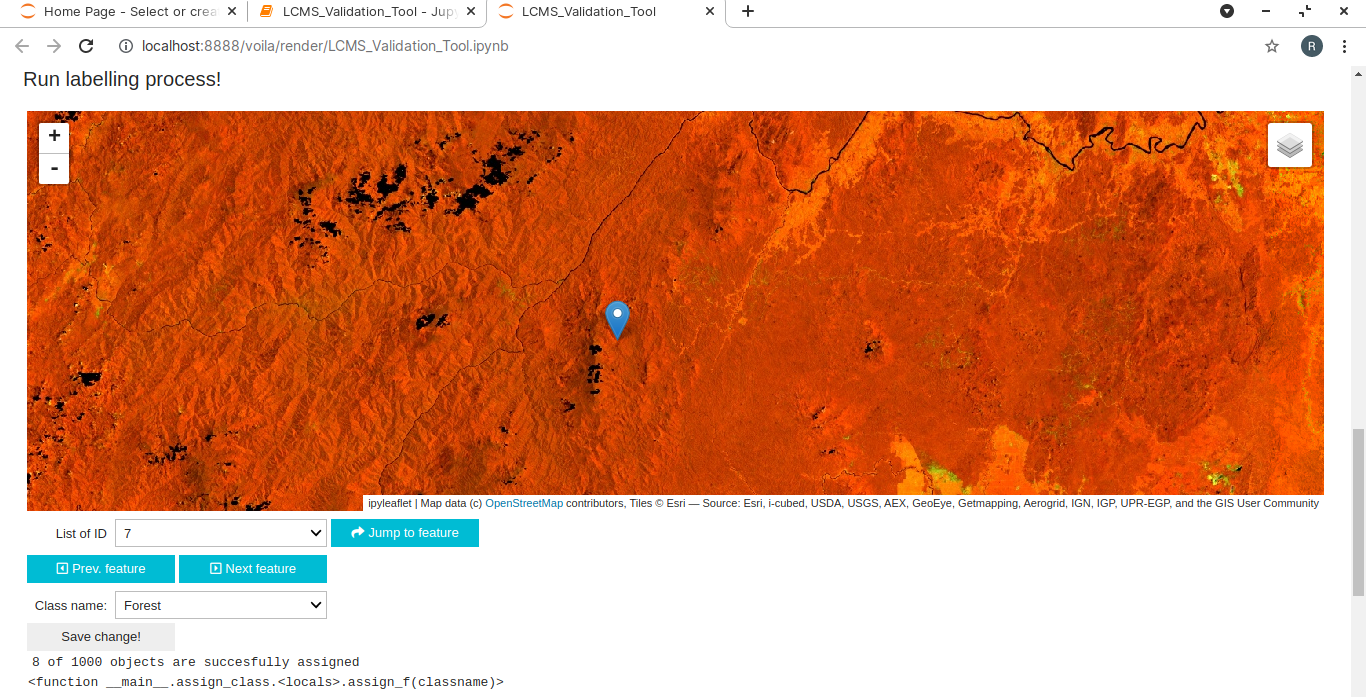
\includegraphics[width = \columnwidth]{ss_1.png}
\caption{\textit{User interface} berbasis \texttt{ipyleaflet} dan \texttt{ipywidgets} untuk labelisasi data secara interaktif}
\end{figure}

\bibliography{library}
\bibliographystyle{ieeetr}

\newpage
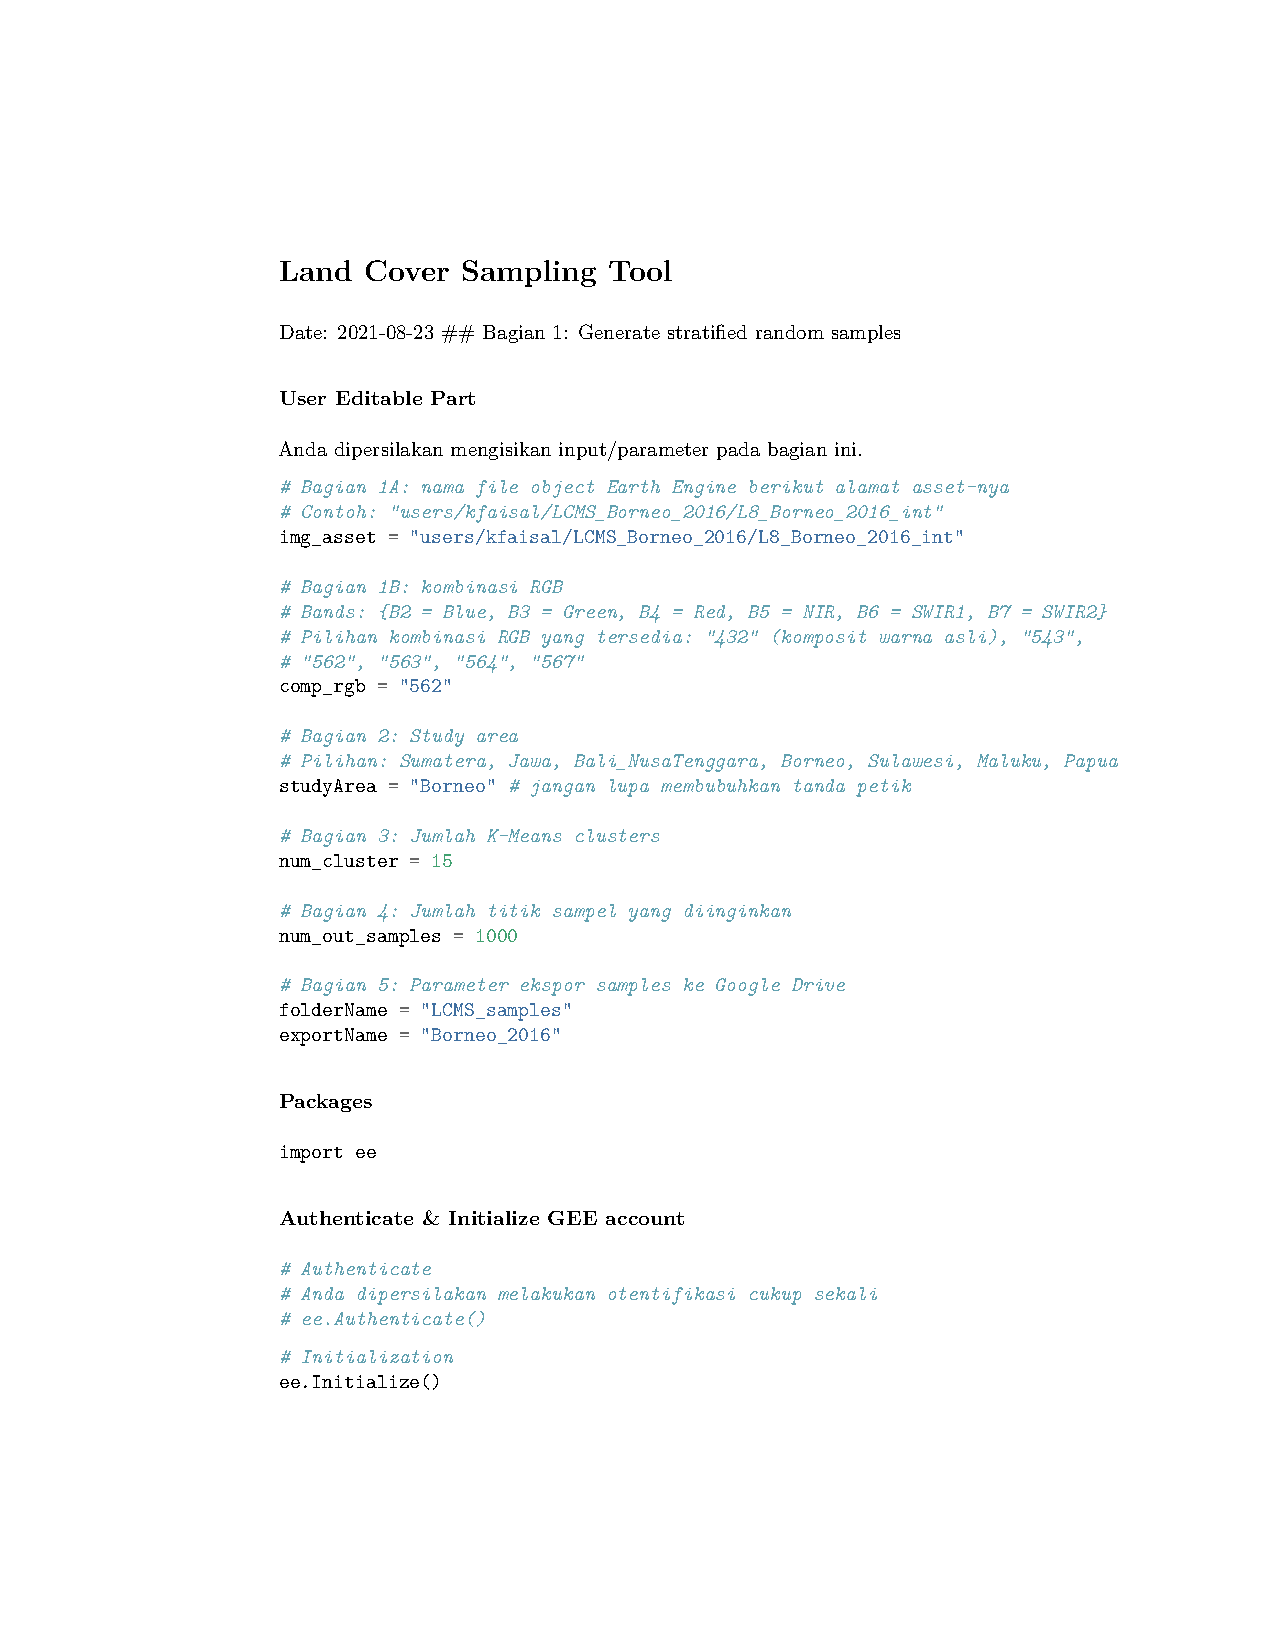
\includepdf[pages = -]{doc1.pdf}

\end{document}